% TODO: train letter classifieru chce dataset z inputu, ktere jsou image
% TODO: zvyraznit syntaxi?
% TODO: best_path_of_word_with_score muze vratit 'nil', pokud zadna takova
% cesta neexistuje. to same find_best_path_of_word_with_score a tranzitivne

\documentclass[a4paper]{article}
\usepackage{fullpage}
\usepackage[utf8]{inputenc}
% \usepackage{amssymb}
% \usepackage{amsmath}
\usepackage[czech]{babel}
\usepackage{listings}
\usepackage{todonotes}
\usepackage{fancyhdr}
\usepackage{listings}
\usepackage{wrapfig}
\usepackage{caption}
\usepackage{subcaption}

\definecolor{string}{rgb}{0.7,0.0,0.0}
\definecolor{comment}{rgb}{0.13,0.54,0.13}
\definecolor{keyword}{rgb}{0.0,0.0,1.0}
\lstset{
% numbers=left,
  language=Ruby,
  frame=single,
  tabsize=2,
  basicstyle=\footnotesize\ttfamily,
  keywordstyle=\color{keyword}\textbf,
  commentstyle=\color{comment}\textit,
  stringstyle=\color{string}
}
\pgfdeclarelayer{background}
\pgfdeclarelayer{foreground}
\pgfsetlayers{background,main,foreground}

\def\datum{15. března 2014}
\def\githuburl{https://github.com/MichalPokorny/rcr.git}

\begin{document}
\title{Uživatelská dokumentace \\ RCR -- OCR knihovna pro Ruby}
\author{Michael Pokorný}
\date{\datum}

\maketitle

\tableofcontents

\section{Základní informace o knihovně}
Účelem knihovny RCR je provádění OCR (Optical Character recognition) nad
předanými obrazovými daty. Jedná se tedy o offline rozpoznávání, neboť
se nepoužívají další informace, jako třeba tlak na pero, pořadí kreslených
čar a podobné. Knihovna dále předpokládá, že vstupní data neobsahují
šum kolem rozpoznávaného písmena. Tento předpoklad se používá k předávání
lepších dat rozpoznávací neuronové síti, avšak to způsobuje problémy,
když se takový šum ve vstupu vyskytne. Je možné knihovnu nastavit tak, aby
tento předpoklad nepoužívala, ale takové nastavení může podstatně snížit
přesnost rozpoznávání.

Testováno bylo pouze rozpoznávání textu složeného z velkých písmen anglické
abecedy. Zdrojový kód knihovny na některých místech implicitně používá tento
předpoklad -- například nástroj \texttt{rcr-train} zatím neumožňuje zadat
jiné povolené znaky.

Knihovna RCR používá sémantické verzování.

Vývoj probíhá přes verzovací systém Git. Repozitář se nachází
na adrese \texttt{\githuburl}.

Používání tohoto softwaru je povoleno pod MIT licencí (viz \texttt{LICENSE.txt}).

\section{Instalace a infrastruktura}
\subsection{Požadavky}
Kromě níže popsaných Ruby gemů (softwarových balíků) požaduje knihovna RCR
nainstalované Ruby verze aspoň 2, grafický toolkit GTK+ 2 a ImageMagick.
Knihovna byla vytvářena s použitím verzovacího systému Git.

\subsubsection{Ruby gemy}
\begin{itemize}
\item \texttt{chunky\_png} umožňuje práci s PNG soubory.
	\texttt{oily\_png} k němu doplňuje optimalizované nativní varianty
	některých operací.
\item \texttt{ruby-fann}: Ruby rozhraní k C knihovně FANN, která implementuje
	základní neuronové sítě. Obsahuje vlastní kopii této knihovny.
\item \texttt{rmagick}: Ruby rozhraní k velmi rozšířené sadě nástrojů pro
	manipulaci s grafikou ImageMagick.
\item \texttt{gtk2}: Ruby bindingy pro GTK+ 2. Používají se v grafických
	komponentách, které knihovna implementuje.
\end{itemize}

Následující gemy jsou vyžadovány pouze pro vývoj knihovny nebo pro instalaci
ze zdrojových kódů.
\begin{itemize}
\item \texttt{bundler}: správce závislostí Ruby gemů
\item \texttt{rake}: Ruby obdoba GNU Make
\end{itemize}

\subsection{Instalace z RubyGems}
Knihovna RCR je Ruby gem.
\todo{napsat postup instalace a zverejnit to}

\subsection{Lokální balíčkování a instalace}
Druhá možnost, jak knihovnu nainstalovat, je vytvořit balíček ze zdrojových
souborů v repozitáři. Lokální kopii repozitáře lze vytvořit spuštěním
\texttt{git clone \githuburl}.

Po nainstalování gemů \texttt{rake} a \texttt{bundler} a spuštění
\texttt{bundle install} se do systému nainstalují potřebné balíky. Poté
stačí spustit \texttt{rake build} v libovolném podadresáři knihovny
k zabalíčkování do adresáře \texttt{pkg}. Příkaz \texttt{rake install} pak
umožňuje tento balík nainstalovat.

\begin{lstlisting}
~ $ git clone https://github.com/MichalPokorny/rcr.git
Cloning into 'rcr'...
remote: Counting objects: 1167, done.
remote: Compressing objects: 100% (460/460), done.
remote: Total 1167 (delta 621), reused 1144 (delta 602)
Receiving objects: 100% (1167/1167), 190.61 KiB | 270.00 KiB/s, done.
Resolving deltas: 100% (621/621), done.
Checking connectivity... done.

~ $ cd rcr

~/rcr $ gem install rake bundler
Fetching: rake-10.1.1.gem (100%)
Successfully installed rake-10.1.1
Parsing documentation for rake-10.1.1
Installing ri documentation for rake-10.1.1
Done installing documentation for rake after 5 seconds
Fetching: bundler-1.5.3.gem (100%)
Successfully installed bundler-1.5.3
Parsing documentation for bundler-1.5.3
Installing ri documentation for bundler-1.5.3
Done installing documentation for bundler after 11 seconds
2 gems installed

~/rcr $ bundle install
\end{lstlisting}
\todo{otestovat ze to jde!!! (tady to v labu selhalo)}
\todo{vypnout ruby syntaxi}

\subsection{Automatické testy}
Knihovna obsahuje sadu automatických testů používajících modul
\texttt{Test::Unit} ze standartní knihovny jazyka Ruby.
Testy se nachází v adresáři \texttt{test} a spouštějí se příkazem
\texttt{rake} nebo \texttt{rake test}. Některá dodatečná data potřebná
ke spuštění testů se nachází v adresáři \texttt{test-data}.

\section{Konfigurace knihovny}
Kvůli jednoduchému sdílení natrénovaných klasifikátorů, vstupních dat
a jiných společných nastavení používá knihovna RCR globální soubor
s konfigurací. Jeho formát je YAML a jeho umístění je \texttt{~/.rcr-config.yml}
na Linuxu, případně obdobný soubor na jiných systémech.
Umožnuje nastavit následující vlastnosti:

\begin{itemize}
\item \texttt{debug}: Booleovská hodnota udávající má-li knihovna vypisovat
	všechna ladící hlášení. Toto se standartně neprovádí.
\item \texttt{data\_path}: Cesta k datům knihovny. Od této cesty se odvozují
	standartní nastavení jiných cest:
	\begin{itemize}
	\item \texttt{trained\_path}: Cesta k natrénovaným modelům - standartně
		\texttt{(data\_path)/trained}.
		\begin{itemize}
		\item \texttt{letter\_classifier\_path}: Cesta k natrénovanému
			klasifikátoru písmen - standartně
			\texttt{(trained\_path)/letter-classifier}.
		\item \texttt{language\_model\_path}: Cesta k natrénovanému
			jazykovému modelu - standartně
			\texttt{(trained\_path)/language-model}.
		\end{itemize}
	\item \texttt{input\_path}: Cesta ke vstupním datům - standartně
		\texttt{(data\_path)/input}.
		\begin{itemize}
		\item \texttt{letter\_inputs\_path}: Cesta ke vstupům s
			písmennými datasety. Formát písmenných datasetů je
			popsán níže. Standartní hodnota je
			\texttt{(input\_path)/letter}.

		\item \texttt{language\_corpus\_path}: Cesta ke korpusu,
			na kterém se trénují jazykové modely.
			Standartně \texttt{(input\_path)/corpus.txt}.

		\item
			\texttt{segmentation\_inputs\_path}: Toto nastavení
			je připraveno pro případné testování a trénování
			segmentace slov na písmena. Protože však nebyl
			žádný testovaný způsob segmentace nedosáhl uspokojivých
			výsledků, není tato možnost v současné verzi knihovny využita.
			Standartní hodnota je \texttt{(input\_path)/segment}.
			Zamýšlený obsah tohoto adresáře jsou jednotlivé příklady
			správně osegmentovaných slov uložené v podadresářích.
			Soubor \texttt{data.png} uvnitř příslušného podadresáře
			by zahrnoval nesegmentované vstupní slovo, zatímto
			soubor \texttt{divided.png} by obsahoval slovo, jehož
			písmena jsou oddělena červenými pixely v místech, kde
			splývají a mají být oddělena, a zelenými pixely v
			místech, kde jedno písmeno netvoří souvislou komponentu
			bitmapy.
		\end{itemize}
	\end{itemize}
\end{itemize}

\begin{figure}[h]
	\centering
	
\includegraphics[width=0.4\textwidth]{divided_sample}
	\caption{Příklad zamýšleného obsahu souboru
	\texttt{divided.png}. Splývající písmena R a O jsou
	oddělena červenými pixely, zatímco dvě komponenty
	písmena D jsou spojeny zelenými pixely.}
\end{figure}

Následuje příklad jednoduchého konfiguračního souboru.
\begin{lstlisting}
---
data_path: /home/prvak/rocnikac/rcr-data/
debug: false
\end{lstlisting}

\subsection{Formát trénovacích dat}
\subsubsection{Písmenné datasety}
Písmenné vstupy knihovny RCR jsou uloženy v podadresářích
cesty \texttt{letter\_inputs\_path}. Každý podadresář obsahuje jeden \uv{datový
blok}. Data takového bloku jsou uložena v jednom obrázku ve formátu PNG,
který je uložen v podadresáři \uv{datového bloku} pod jménem \texttt{data.png}.
Každý takový obrázek se skládá ze stejně velkých obdélníkových buněk. Buňka
obsahuje jedno vstupní písmeno. Stejná písmena jsou v jednom sloupci.

Kromě obrázku se vstupy trénovací data také zahrnují deskriptor, který popisuje
jejich formát a uložené znaky. Jedná se o YAML soubor pojmenovaný
\texttt{data.yml}. Obsahuje volitelně parametry \texttt{cell\_height} a
\texttt{source} a povinně parametr \texttt{segments}.
Parametr \texttt{cell\_height} uvádí výšku buněk v obrázku, pokud nejsou
čtvercové. Parametr \texttt{source} je určený k případnému budoucímu oddělování
datasetů různého původu (například naskenované dokumenty, datasety vytvořené
z fontů na počítači, atd.).
Povinný parametr \texttt{segments} obsahuje popis písmen ve sloupcích datasetu.
Tento popis se skládá z bloků písmen, která po sobě následují ve znakové sadě
ASCII. Každý takový blok je daný svým začátkem (\texttt{first}) a koncem
(\texttt{last}).

\begin{figure}[h]
        \centering
        \begin{subfigure}[b]{0.5\textwidth}
		\centering
                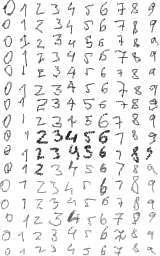
\includegraphics[width=0.6\textwidth]{letter_dataset_sample}
		\caption{\texttt{data.png}}
        \end{subfigure}%
        ~ %add desired spacing between images, e. g. ~, \quad, \qquad, \hfill etc.
          %(or a blank line to force the subfigure onto a new line)
        \begin{subfigure}[b]{0.5\textwidth}
\begin{lstlisting}
segments:
        -
                first: '0'
                last: '9'

source: human_freehand
\end{lstlisting}
		\caption{\texttt{data.yml}}
        \end{subfigure}
        \caption{Ilustrace formátu písmenných vstupů}
\end{figure}

\section{Rozhraní pro Ruby}

\subsection{Zjednodušené rozhraní}
Aby nebylo potřeba při každém použití knihovny složitě vytvářet klasifikátory,
obsahuje knihovna i zjednodušené rozhraní. Toto rozhraní umožňuje jednoduše
používat obvyklé funkce a jedním příkazem vytvořit komponenty knihovny podle
základní konfigurace.

Toto rozhraní se importuje příkazem \texttt{require 'rcr/easy'}.

\subsubsection{Načítání obrazu}
K jednoduchému načítání obrazových dat k použití knihovnou RCR slouží metody
\texttt{RCR.load\_image} a \texttt{RCR.load\_image\_from\_blob}. Metoda
\texttt{RCR.load\_image} bere jako jediný parametr cestu k souboru k načtení.
Metoda \texttt{RCR.load\_image\_from\_blob} oproti tomu bere jako svůj parametr
obsah tohoto souboru.
\begin{lstlisting}
image = RCR.load_image("letter.png")
image2 = RCR.load_image_from_blob(File.read("letter.png"))
\end{lstlisting}

\subsubsection{Vytváření komponent dle standartní konfigurace}
Metody \texttt{RCR.build\_letter\_classifier} a
\texttt{RCR.build\_language\_model} nahrají klasifikátor písmen, respektive jazykový model
dle standartní konfigurace. Těmto metodám je možné předat jako argument
\texttt{Hash}, kterým lze tuto konfiguraci upravit.
\begin{lstlisting}
classifier = RCR.build_letter_classifier(letter_classifier_path: "/tmp/classifier")
model = RCR.build_language_model
\end{lstlisting}

Díky těmto metodám je jednoduché vyrobit a používat komponenty knihovny
bez hluboké znalosti jejich funkcí:
\begin{lstlisting}
classifier = RCR.build_letter_classifier
image = RCR.load_image("letter.png")
puts "Detected letter: #{classifier.classify(image)}"
\end{lstlisting}

Metoda \texttt{RCR.build\_word\_segmentator} zatím vždy vyrábí instanci
\texttt{RCR::WordSegmentator::HeuristicOversegmentation} založenou na
oversegmenteru \texttt{RCR::HeuristicOversegmenter::LocalMinima}. Jazykový model
a klasifikátor písmen je do tohoto segmentátoru dodaný podle standartní
konfigurace.

\subsection{Práce s obrazem}
Knihovna RCR obsahuje několik tříd, které obalují různé zdroje obrazových dat
společným rozhraním.

\subsubsection{\texttt{RCR::Data::Image}: základní reprezentace obrazu}
Obrázky uložené jako soubory jdou reprezentovat třídou
\texttt{RCR::Data::Image}. Interně tato třída využívá obdobné třídy knihovny
\texttt{chunky\_png} nebo \texttt{RMagick}.
Tato komponenta se načítá příkazem \texttt{require 'rcr/data/image'}.

Způsoby vytváření instancí této třídy určené pro vnějšího uživatele jsou tři:
\begin{itemize}
\item \texttt{RCR::Data::Image.load} přijímá jeden parametr, který je cesta k
souboru:
% ImageTest#test_loading_works
\begin{lstlisting}
image = RCR::Data::Image.load("image.png")
\end{lstlisting}
\item \texttt{RCR::Data::Image.from\_blob} umožňuje načtení obrázku přímo z
paměti:
% ImageTest#test_blob_loading_works
\begin{lstlisting}
data = File.read("image.png")
image = RCR::Data::Image.from_blob(data)
\end{lstlisting}
\item \texttt{RCR::Data::Image.from\_pixel\_array} načítá obrázek reprezentovaný
jako dvourozměrné pole trojic osmibitových RGB hodnot:
% ImageTest#test_pixel_array_loading_works
\begin{lstlisting}
data = [
	[ [11, 11, 11], [21, 21, 21], [31, 31, 31] ],
	[ [12, 12, 12], [22, 22, 22], [32, 32, 32] ],
]
array_image = RCR::Data::Image.from_pixel_array(data)
# [image.width, image.height] == [3, 2]
\end{lstlisting}
\end{itemize}

Samotný konstruktor je možné použít pouze s parametrem typu
\texttt{ChunkyPNG::Canvas} nebo \texttt{Magick::Image}. Takto použitý
konstruktor vytvoří instanci obalující předaný obrázek.

Vlastnosti \texttt{width} a \texttt{height} udávají šířku a výšku obrázku.
Indexování po souřadnicích umožňuje přistupovat k pixelům, které jsou přístupné
jako osmibitové RGB trojice:
% ImageTest#test_pixel_array_loading_works
\begin{lstlisting}
pixel = array_image[2, 1]
# pixel == [32, 32, 32]
\end{lstlisting}

Jako alternativní rozhraní k přístupu k pixelům se dá použít metoda
\texttt{pixels}. Vrací enumerátor, který vrací RGB trojice v pořadí
po řádcích. Na tomto objektu je možné používat obvyklé metody jako
\texttt{each}, \texttt{map}, atd. aniž by bylo nutné bezpodmínečně
vytvářet pole všech pixelů jako Ruby objekt.

Metoda \texttt{\#save} uloží obrázek do zadaného souboru:
% ImageTest#test_pixel_array_loading_works
\begin{lstlisting}
array_image.save("array_image.png")
\end{lstlisting}

Zavolání metody \texttt{\#crop} vrátí oříznutý obraz. V parametrech přijímá
postupně minimální X a Y souřadnici oříznuté oblasti a její šířku a výšku.
Implicitně tato metoda vrací línou reprezentaci obrazu. Tomu se dá zabránit
předáním parametru \texttt{lazy} s hodnotou \texttt{false}.
% TODO: ukazka?

Metoda \texttt{\#crop\_by\_columns} je pomocný obal nad metodou \texttt{\#crop}
určený k rozřezávání písmenných datasetů na jednotlivá písmena. Každý dataset
se skládá ze stejně velkých obdélníkových oblastí. Každá z nich obsahuje jedno
písmeno. Vstupy se stejným písmenem se nacházejí ve stejném sloupci.
První parametr metody udává počet stejně širokých sloupců v obrazu.
Druhý nepovinný parametr obsahuje výšku každé buňky; není-li uveden, použije
se jako výška buňky šířka sloupců. Nepovinně je možné předat parametr
\texttt{lazy} s hodnotou \texttt{false}, čímž se zabrání vrácení líné
reprezentace obrazu. Výsledek této metody je pole, jehož prvky jsou vyříznuté
buňky každého sloupce (pro sloupce obsahující písmena A, B a C například
\texttt{[ [A1, A2], [B1, B2], [C1, C2] ]}).
% TODO: ukazka?

Obrázek jde zmenšit na danou velikost metodou \texttt{\#scale}, případně
\texttt{\#scale!}. Její parametry jsou šířka a výška výsledku.
% ImageTest#test_pixel_array_loading_works
\begin{lstlisting}
scaled = array_image.scale(20, 20)
\end{lstlisting}
Metoda \texttt{\#border\_to\_and\_resize\_to\_fit!} provádí podobnou operaci,
avšak zachovává přitom poměr stran. Obraz se zvětší tak, aby byl co největší,
a přitom obsažený v obdélníku dané velikosti. Zbylé místo se doplní bílou
barvou.

Metody \texttt{\#guillotine} a \texttt{\#guillotine!} z obrázku ořezávají
bílé okraje. Nepřijímají žádné parametry.

Metoda \texttt{\#mutate} je určena pro umělé zvětšování datasetu. Vrátí obrázek
po drobné náhodné afinní transformaci (změna velikosti obou rozměrů na 90--110\%,
otočení o -11,25 až $11,25^\circ$).

Především k ladícím účelům slouží metoda \texttt{\#draw\_rectangle!}, která na
obraz nakreslí obdélník. Pořadí parametrů je následující: X, Y souřadnice levého
horního rohu, X, Y souřadnice pravého dolního rohu, barva okraje, barva vnitřku.
Standartní barva okraje je černá a standartní barva vnitřku je průhledná
(vnitřek se tedy nevykreslí). Barvy jsou objekty typu \texttt{ChunkyPNG::Color}.
Modul \texttt{RCR::Data::Image::Color} obsahuje zkratky \texttt{BLACK},
\texttt{RED}, \texttt{GREEN}, \texttt{BLUE} a \texttt{TRANSPARENT}.
% ImageTest#test_pixel_array_loading_works
\begin{lstlisting}
scaled.draw_rectangle!(
  5, 5, 15, 15,
  RCR::Data::Image::Color::RED, RCR::Data::Image::Color::BLUE
)
\end{lstlisting}

\subsubsection{\texttt{RCR::Data::LazyImage}: líná reprezentace obrazu}
Aby se omezil čas strávený kopírováním obrazových dat, která jsou od sebe
odvozena jednoduchými transformacemi, obsahuje knihovna několik tříd, které
se chovají podobně jako \texttt{RCR::Data::Image}, ale přitom reprezentují
jenom nějakou jednoduchou transformaci provedenou nad jiným obrazovým objektem.

K používání uživatelem je určena třída \texttt{RCR::Data::LazyImage}.
Obaluje buď línou reprezentaci obrazu, nebo obraz, a zjistí-li, že uložená
líná reprezentace obrazu neimplementuje nějakou z volaných metod, automaticky
převede vnitřní objekt na obraz. Tím pádem je možné nad touto třídou používat
libovolné metody třídy \texttt{RCR::Data::Image}, i když se jedná ve skutečnosti
jenom o objekt reprezentující \uv{recept na výrobu obrazu}.

Mezi tyto \uv{recepty na výrobu obrazu} patří třídy
\texttt{RCR::Data::MergedImagelike} (ze dvou vstupních obrázků vrátí pixel
s nižší světlostí), \texttt{RCR::Data::CroppedImagelike} (chová se jako
oříznutá oblast z jiného obrázku), \texttt{RCR::Data::CairoImagelike}
(reprezentuje obraz importovaný z grafické knihovny Cairo) a nakonec
\texttt{RCR::Data::MaskedImagelike} (pixely obrazu vybrané upravitelnou
bitmapovou maskou ukazuje jako bílé).
Všechny tyto třídy dědí od \texttt{RCR::Data::Imagelike}.

\subsection{Neuronové sítě}
\subsubsection{\texttt{RCR::Data::NeuralNetInput}: vstup pro neuronovou síť}
Třída \texttt{RCR::Data::NeuralNetInput} se importuje pomocí \texttt{require
'rcr/data/neural\_net\_input'}. Tato třída se používá všude v knihovně, kde
je se pracuje s daty, která půjdou na vstup neuronové síti. Účelem třídy
je omezit málo restriktivní rozhraní, které by nabízelo použití jiných datových
typů (například pole). Tato třída znesnadňuje svým uživatelům provádět operace,
které by mohly porušit invariant \uv{jedná se o validní vstup neuronové sítě}.
Pokud by například chyba v kódu způsobila, že se neuronové síti předá pole
obsahující kromě čísel také položky typu \texttt{String}, mohla by se projevit
velice hluboko v kódu RCR. Takto se tato logická chyba objeví dříve: ve chvíli,
kdy by došlo k pokusu vytvořit \texttt{RCR::Data::NeuralNetInput} z pole,
jehož položky nejsou pouze čísla.

Veřejné rozhraní \texttt{RCR::Data::NeuralNetInput} se skládá z konstruktoru a
metod \texttt{\#==}, \texttt{NeuralNetInput.concat}, \texttt{\#size} a \texttt{\#data}.

Konstruktor bere jako jediný parametr \texttt{Array}-like objekt obsahující
prvky typu \texttt{Float}. Vložení jiných datových typů (včetně jiných číselných
typů jako \texttt{BigDecimal} nebo \texttt{Integer}) je chyba.
% NeuralNetInputTest#test_basic
\begin{lstlisting}
input = RCR::Data::NeuralNetInput.new([0.1, 0.2, 0.3])
\end{lstlisting}

Metoda \texttt{\#==} podle své standartní sémantiky porovnává dva objekty typu
\texttt{RCR::Data::NeuralNetInput}. Platí zde obvyklé problémy s aritmetikou
v plovoucí čárce.
% NeuralNetInputTest#test_basic
\begin{lstlisting}
input == RCR::Data::NeuralNetInput.new([0.1, 0.2, 0.3]) # true
\end{lstlisting}

Metoda \texttt{NeuralNetInput.concat} spojuje dva nebo více vstupů za sebe:
% NeuralNetInputTest#test_basic
\begin{lstlisting}
NeuralNetInput.concat(input, RCR::Data::NeuralNetInput.new([0.4, 0.5])) ==
  RCR::Data::NeuralNetInput([0.1, 0.2, 0.3, 0.4, 0.5])
\end{lstlisting}

% NeuralNetInputTest#test_basic
Obsah této třídy je možné získat jako pole pomocí metody \texttt{\#data}.
Tato metoda je však určena především pro vnitřní účely knihovny RCR.
\begin{lstlisting}
input.data == [0.1, 0.2, 0.3] # true
\end{lstlisting}

\subsubsection{\texttt{RCR::Data::Dataset}: abstrakce nad datasety}
Třída \texttt{RCR::Data::Dataset} se importuje pomocí \texttt{require
'rcr/data/dataset'}. Jedná se o abstrakci nad datasetem: uspořádanou
množinou párů \uv{vstup - očekávaný výstup}. Tato třída se nepoužívá jen
při práci s neuronovými sítěmi, ale i například při práci s klasifikátory.

Konstruktor této třídy přijímá buď parametr typu \texttt{Array}, nebo parametr
typu \texttt{Hash}.

Parametr typu \texttt{Array} se interpretuje jako seznam
párů \uv{vstup - očekávaný výstup}:
% RCR::Data::DatasetTest#test_basic
\begin{lstlisting}
# Dataset pro funkci 'y = x0 + x1'
dataset = RCR::Data::Dataset.new([
  [[0.1, 0.1], 0.2], [[0.3, 0.5], 0.8], [[-0.5, 0.5], 0.0], [[0.1, -0.3], -0.2]
])
\end{lstlisting}

Tato třída kontroluje konzistenci datových typů vstupů a očekávaných výstupů.
K zjištění uloženého typu vstupů, respektive výstupů je možné použít metody
\texttt{\#input\_type} a \texttt{\#expected\_output\_type}.
% RCR::Data::DatasetTest#test_basic
\begin{lstlisting}
dataset.input_type == Array && dataset.expected_output_type == Float # true
\end{lstlisting}

Předá-li se konstruktoru parametr typu \texttt{Hash}, jsou jeho
klíče interpretovány jako očekávané výsledky a hodnoty jako
pole vstupů, které mají dát daný výsledek:
% RCR::Data::DatasetTest#test_basic
\begin{lstlisting}
# Dataset pro funkci 'y = x0 + x1'
dataset2 = RCR::Data::Dataset.new({
  0.0 => [[-0.1, 0.1], [0.0, 0.0], [0.5, -0.5]],
  0.5 => [[-0.1, 0.6], [0.4, 0.1], [0.2, 0.3]],
  -0.5 => [[-0.2, -0.3], [0.2, -0.7], [-0.9, 0.4]],
})
\end{lstlisting}

Třída implementuje funkce \texttt{\#empty?}, \texttt{\#shuffle!} a
\texttt{\#size} obdobným způsobem jako standartní třída \texttt{Array}
(tedy dotaz na prázdnost, náhodné přeházení na místě a dotaz na počet párů
vstup-výstup).

Funkce \texttt{\#each} iteruje přes všechny páry klíč-hodnota:
% TODO: test
\begin{lstlisting}
# [-0.1, 0.1] -> 0.0, [0.0, 0.0] -> 0.0, ...
text = ""
dataset2.each { |pair| text << "#{pair.first.inspect} -> #{pair.last}, " }
puts text
\end{lstlisting}

Pomocí metody \texttt{\#insert} lze vkládat nová data:
% TODO: test
\begin{lstlisting}
dataset.insert([0.7, 0.2], 0.9)
\end{lstlisting}

Funkce \texttt{\#split} s volitelným pojmenovaným parametrem \texttt{threshold}
rozdělí instanci na dva kusy v poměru daném tímto parametrem. Jeho standartní
hodnota je \texttt{0.8}. Tato hodnota způsobí, že první vrácený poddataset bude
přibližně $4\times$ větší než druhý.
Tato funkce se dá použít například na pohodlné rozdělení na trénovací a
testovací data:
% TODO: test
\begin{lstlisting}
train, test = dataset2.split(threshold: 0.75)
\end{lstlisting}

Metoda \texttt{\#restrict\_expected\_outputs} je určena pro odstranění nechtěných klíčů
z datasetu. Dá se použít například máme-li dataset obsahující správné klasifikace
obrázků písmen a čísel, ale chceme-li trénovat pouze klasifikátor na čísla.
Obsah původního datasetu zůstane nezměněný, dataset s méně klíči se pouze vrátí.
Varianta \texttt{\#restrict\_expected\_outputs!} naopak původní objekt změní.
\begin{lstlisting}
number_dataset = whole_dataset.restrict_expected_outputs('0'..'9')
\end{lstlisting}

Pomocí metody \texttt{\#to\_xs\_ys\_arrays} lze z datasetu získat dvojici polí,
kde první z nich obsahuje vstupy a druhé obsahuje na stejných indexech příslušné
očekávané výstupy. Tato dvojice polí se hodí například pro předávání dat do
knihovny FANN.

Metody \texttt{\#transform\_inputs} a \texttt{\#transform\_expected\_outputs} transformují
přes předaný blok všechny vstupy, respektive očekávané výstupy, a vrátí změněný
objekt \texttt{Dataset}. Původní objekt zůstane nezměněný.
Varianty těchto metod s vykřičníkem (\texttt{\#transform\_inputs!} a
\texttt{\#transform\_expected\_outputs!}) oproti tomu změní původní objekt.
% DatasetTest#test_transformations
\begin{lstlisting}
dataset = RCR::Data::Dataset.new([[1, 5], [2, 10], [3, 15]])
dataset2 = dataset.transform_inputs { |x| x * 5 }.
  transform_expected_outputs { |y| y / 5 }
dataset2 == RCR::Data::Dataset.new([[5, 1], [10, 2], [15, 3]]) # true
\end{lstlisting}

Metoda \texttt{\#to\_fann\_dataset} vrací analogickou třídu typu
\texttt{RubyFann::TrainData}. Tato metoda je použitelná pouze jsou-li vstupy i
očekávané výstupy pole čísel. Výsledek lze předat k použití knihovně RubyFann.

\subsubsection{\texttt{RCR::NeuralNet}: neuronové sítě}
Knihovna RCR používá jednoduché feed-forward neuronové sítě. Samotná
implementace algoritmů se nachází v knihovně FANN (Fast Artificial Neural % TODO: reference
Network Library). RCR také používá RubyFann, což je rozhraní nad touto knihovnou
pro jazyk Ruby (samotná knihovna FANN je v jazyce C). Kvůli menším závislostem
na FANN a kvůli méně pohodlnému návrhu rozhraní RubyFann byla vytvořena další
vrstva abstrakce.

Příslušná třída se jmenuje \texttt{RCR::NeuralNet} a je možné ji naimportovat
pomocí \texttt{require 'rcr/neural\_net'}.

Konstruktor této třídy pouze obalí existující objekt reprezentující neuronovou
síť v RubyFann:
\begin{lstlisting}
fann_net = RubyFann::Standard.new(num_inputs: 10, num_outputs: 5,
  hidden_neurons: [8, 8, 8])
net = RCR::NeuralNet.new(fann_net, 10, 5)
\end{lstlisting}

Zavolání \texttt{NeuralNet.create} je zkratka za vytvoření RubyFann neuronové
sítě a její obalení:
\begin{lstlisting}
net = RCR::NeuralNet.create(num_inputs: 10, num_outputs: 5,
  hidden_neurons: [8, 8, 8])
\end{lstlisting}

Metoda \texttt{train} natrénuje neuronovou síť na každém vzoru uloženém
v předaném datasetu. Dataset musí mít typ vstupů \texttt{RCR::Data::NeuralNetInput} a
výstupy musí být pole čísel. Tato metoda provede pouze jedno kolo tréningu.
K získání použitelných výsledků je potřeba volání této metody opakovat.
% NeuralNetTest#test_train_xor
\begin{lstlisting}
# dataset pro funkci XOR
dataset = RCR::Data::Dataset.new([[[0, 0], 0], [[0, 1], 1], [[1, 0], 1], [[1, 1], 0]]).
  transform_inputs { |x| RCR::Data::NeuralNetInput.new(x.map(&:to_f)) }.
  transform_expected_outputs { |y| [y.to_f] }
net = RCR::NeuralNet.create(num_inputs: 2, num_outputs: 1,
  hidden_neurons: [4, 4])
1000.times { net.train(dataset) }
\end{lstlisting}

Nejdůležitější metoda třídy \texttt{RCR::NeuralNet} se jmenuje \texttt{\#run}.
Tato metoda předá neuronové síti vstup typu \texttt{RCR::Data::NeuralNetInput} a
vrátí pole výstupů neuronů na poslední vrstvě.
% NeuralNetTest#test_train_xor
\begin{lstlisting}
output = net.run(RCR::Data::NeuralNetInput.new([0.9, 0.8]))
output[0] < 0.2 # true

output = net.run(RCR::Data::NeuralNetInput.new([0.1, 0.9]))
output[0] > 0.8 # true
\end{lstlisting}

\todo{image transformery}

\subsection{\texttt{RCR::Classifier}: klasifikátory}

Klasifikace je úloha předpovídání diskrétní kategorie daného vstupu na základě
trénovacích dat. Knihovny samotná je používá pouze k detekci napsaného písmena,
ale je možné je použít i samostatně k jiným účelům. Implementován je pouze jeden
typ klasifikátoru, a to klasifikátor založený na neuronových sítích
(\texttt{RCR::NeuralNet}).

Třída \texttt{RCR::Classifier::Base} je zamýšlena jako předek všech
klasifikátorů. Aby byly následující příklady
kódu spustitelné, používají \texttt{RCR::Classifier::Neural}. Jsou nicméně
míněny jako specifikace společného rozhraní, které by měl splňovat i případný
jiný typ klasifikátoru odvozený od \texttt{RCR::Classifier::Base}.

Konstruktor třídy přijímá nejvýše jeden parametr, který je
interpretován jako seznam tříd ke klasifikaci. Je však určený k tomu,
aby byl zavolán konstruktorem odvozeného konkrétního klasifikátoru.
Odvozený klasifikátor může vyžadovat další parametry.

Tento seznam tříd je pak dostupný přes metodu \texttt{\#classes}.
Klasifikátor dále musí implementovat metody \texttt{\#classify},
\texttt{\#classify\_with\_score}, \texttt{\#classify\_with\_alternatives},
\texttt{\#train} a \texttt{\#evaluate}.

Klasifikátor očekává vstupy zformátované jako pole čísel.
Metody \texttt{\#classify}, \texttt{\#classify\_with\_score} a
\texttt{\#classify\_with\_alternatives} vrací výsledky klasifikace
na jednom vstupu a vrací různé druhy výsledků. Metoda \texttt{\#classify}
vrátí pouze předpovězenou kategorii, zatímco \texttt{classify\_with\_score}
vrátí pár (předpovězená kategorie, její skóre).
\texttt{classify\_with\_alternatives} nakonec vrátí \texttt{Hash}, jehož
klíče jsou kategorie a hodnoty jsou relativní skóre daných kategorií.
Všechna skóre musí být normalizována tak, aby součet skóre přes všechny
vrácené alternativy byl 1. Metoda \texttt{classify\_with\_score} musí
tuto podmínku také splňovat.

Odvozené klasifikátory nemusí implementovat všechny tyto metody.
Stačí doplnit \texttt{classify\_with\_alternatives} -- všechny ostatní
klasifikační metody mají v \texttt{RCR::Classifier::Base} odvozenou
standartní implementaci. Bylo-li by však určení skóre všech kategorií
pomalé, může být užitečné poskytnout rychlejší implementaci v konkrétním
klasifikátoru.

Metody \texttt{\#train} a \texttt{\#evaluate} přijímají \texttt{Dataset}.
\texttt{\#train} natrénuje klasifikátor podle daných dat a \texttt{\#evaluate}
vrátí úspěšnost klasifikátoru (číslo mezi 0 a 1).

% TODO: test a priklady kodu
\subsubsection{\texttt{RCR::Classifier::Neural}: klasifikátory založené na
neuronových sítích}
Tato třída se nachází v modulu \texttt{'rcr/classifier/neural'}.
Tyto klasifikátory obsahují uvnitř neuronovou síť, která přijímá stejné vstupy
jako klasifikátor. Jejím výstupem je pro každou kategorii jedno číslo, které
je interpretováno jako relativní skóre. Klasifikátor pak předpoví tu kategorii,
která má toto skóre nejvyšší.

% TODO: test a priklad
Vyrábí se pomocí metody \texttt{RCR::Classifier::Neural.create}. Její parametry
\texttt{num\_inputs} a \texttt{hidden\_neurons} odpovídají příslušným parametrům
metody \texttt{RCR::NeuralNet.create}. Parametr \texttt{classes} obsahuje seznam
kategorií.
% NeuralFunctionalTest#test_create
\begin{lstlisting}
classifier = RCR::Classifier::Neural.create(
  num_inputs: 3,
  hidden_neurons: [3, 3],
  classes: [1, 2, 3]
)
\end{lstlisting}

Metoda \texttt{\#train} kromě datasetu obsahuje přijímá také jako parametr
\texttt{generations} počet iterací trénování (není-li uveden, použije se 1000).

\texttt{dataset\_split}
\todo{dopsat tenhle kus}

\subsection{\texttt{RCR::FeatureExtractor}}
Třídy ve jmenném prostoru \texttt{RCR::FeatureExtractor} převádí obraz (objekty
typu \texttt{RCR::Data::Image}) na data vhodná jako vstup ostatních komponent
knihovny (klasifikátorů, neuronových sítí atd.).
Všechny tyto třídy implementují metody \texttt{\#extract\_features} a
\texttt{\#output\_size}. Metoda \texttt{\#extract\_features} jako parametr
přijímá obraz a vrací pole čísel velikosti \texttt{\#output\_size}.
Velikost výstupu není závislá na vstupním obrazu.

Třída \texttt{RCR::FeatureExtractor::ContentAspectRatio} převádí obraz na jediné
číslo, které vyjadřuje poměr stran neprázdné části obrazu. Vstupní obraz se
ořízne na neprázdnou část a vrátí se poměr šířky a součtu šířky a výšky výsledku.

Druhá třída v tomto jmenném prostoru je \texttt{RCR::FeatureExtractor::RawImage}.
Její výstup je vyjádření samotného obsahu obrazu. Obraz se před převedením na
čísla volitelně ořízne na neprázdnou část, pak se vždy zmenší na jednotnou velikost
(buď se zachováním poměru stran, nebo bez něj) a nakonec se volitelně může
normalizovat kontrast obrazu. (Normalizace kontrastu znamená přepočítání
výsledku tak, aby se rozkládal přes celý interval $[0;1]$.)

První dva parametry konstruktoru vyjadřují šířku a výšku, na kterou se bude
vstup zmenšovat. Další volitelné parametry \texttt{guillotine},
\texttt{forget\_aspect\_ratio} a \texttt{normalize\_contrast} určují, má-li
se provádět oříznutí na neprázdný obsah, má-li se vstup zmenšovat bez zachování
poměru stran a má-li být nakonec vykonána normalizace kontrastu.

\subsection{\texttt{RCR::LetterClassifier}}
Tento jmenný prostor obsahuje třídy, které obalují klasifikátory pro potřeby
OCR jednotlivých písmen. Tyto třídy implementují API analogické k obecným
klasifikátorům (tedy metody \texttt{\#train}, \texttt{\#evaluate}, \texttt{\#classify},
\texttt{\#classify\_with\_score} a \texttt{\#classify\_with\_alternatives}),
ale očekávají jako své vstupy instance \texttt{RCR::Data::Image} (nebo línou
reprezentaci obrazu), případně datasety obsahující tyto instance.

Třída \texttt{RCR::LetterClassifier::Base} je předek všech ostatních tříd
tohoto jmenného prostoru.

\subsubsection{\texttt{RCR::LetterClassifierNeural}}
Tento klasifikátor písmen používá \texttt{RCR::Classifier::Neural}.
Před předáním obrazu neuronové síti se nad nimi provede nastavitelná
transformace (například lze síti volitelně předat poměr stran obsahu
obrazu).

Před natrénováním této třídy je potřeba nejdříve zavolat metodu
\texttt{\#start\_anew} a předat ji v parametrech \texttt{transformer},
\texttt{allowed\_chars} a \texttt{hidden\_neurons} převodník obrazu
na data (popsáno níže), množinu povolených znaků a velikosti skrytých
vrstev neuronové sítě.

Metoda \texttt{\#train} přijímá navíc parametr \texttt{generations},
kterým je možné měnit dobu trénování neuronové sítě. Standartní hodnota
je 1000.

Příklad použití včetně vyrobení převodníku obrazu na data:
\begin{lstlisting}
input_transformer = LetterClassifier::InputTransformer::Basic.new(
	FeatureExtractor::RawImage.new(
		8, 8, guillotine: true, forget_aspect_ratio: true, normalize_contrast: true
	)
)
classifier = Neural.new
# inputs = ...
dataset = LetterClassifier.load_inputs(inputs)
classifier.start_anew(transformer: input_transformer, allowed_chars: ('0'..'9'))
classifier.train(dataset, generations: 20)
classifier
\end{lstlisting}

\subsection{\texttt{RCR::HeuristicOversegmenter}}
\todo{napsat}

\subsection{\texttt{RCR::WordSegmentator}}
Tento modul obsahuje dva jednoduché rozdělovače slov na písmena.
Jejich základní API tvoří metoda \texttt{\#segment}, která přijímá obraz k
rozdělení a vrací jeho segmentaci (instanci \texttt{RCR::Data::Segmentation}).
\todo{zdokumentovat RCR::Data::Segmentation}

\subsubsection{\texttt{RCR::WordSegmentator::SimpleContiguousParts}}
Tato třída vstup rozděluje na souvislé komponenty.
\todo{dopsat}

\subsection{\texttt{RCR::MarkovChain}: Markovské řetězce}
Knihovna RCR používá Markovské řetězce jako primitiva uvnitř jazykových modelů.
Příslušná třída se nazývá \texttt{RCR::MarkovChain} a importuje se příkazem
\texttt{require 'rcr/markov\_chain'}. Ačkoliv tento popis mluví o Markovských
řetězcích nad písmeny, je tato třída naprogramována obecně -- může pracovat nad
libovolnými objekty.

Markovský řetězec je interně reprezentovaný jako \texttt{Hash}, ve kterém klíče
jsou možné kontexty a hodnoty jsou \texttt{Hash}e, jejichž klíče jsou možná
pokračování a hodnoty jsou jejich pravděpodobnosti. Součet pravděpodobností
pokračování musí být 1.

Konstruktor Markovského řetězce přijímá jako první parametr svou hloubku (0
znamená triviální Markovský řetězec držící jenom relativní četnosti písmen, 1
znamená počítání pravděpodobnosti podle jednoho předcházejícího písmena, atd.).
Druhý volitelný parametr je interní \texttt{Hash}. Je-li uveden, bude tento
řetězec inicializován do příslušného stavu.
% TODO: test
\begin{lstlisting}
mc = MarkovChain.new(2)
mc2 = MarkovChain.new(2, { "AB" => { "C" => 0.7, "A" => 0.3 }, ... })
\end{lstlisting}

Metoda \texttt{\#train} zahodí obsah Markovského řetězce a natrénuje jej na
daném textu nebo poli.
% MarkovChainTest#test_docs
\begin{lstlisting}
mc.train("ABC ABD ABA ABC ABC")
\end{lstlisting}

Metoda \texttt{\#score} vrací relativní skóre (pravděpodobnost) daného
pokračování dle kontextu, případně \texttt{nil} pokud tento Markovský řetězec
na toto pokračování nebyl natrénován. První parametr je kontext a druhý parametr
je pokračování k ohodnocení. Kontext může být jak pole, tak řetězec.
% MarkovChainTest#test_docs
\begin{lstlisting}
mc.score("AB", "C") # 0.6
\end{lstlisting}

\subsection{\texttt{RCR::LanguageModel}: jazykové modely}
Jazykové modely jsou komponenty, které umí klasifikátoru \uv{radit}
reálné šance, že jeho hypotézy jsou správné: text,
který by mohl být po písmenech přečtený jako \texttt{T0PA2} (s číslem
\texttt{0}), může být vhodným modelem opraven na \texttt{TOPAZ}, protože
model může vědět, že je nepravděpodobné, aby se v jednom slově mixovaly
číslice a písmena (nebo může například udržovat množinu slov, která
přijímá).

\todo{definice spolecneho API}

\subsubsection{\texttt{RCR::LanguageModel::MarkovChain}: jazykové modely
založené na Markovských řetězcích}
\todo{napsat}

\subsection{\texttt{RCR::GUI}: grafické komponenty}
\todo{napsat}
\subsubsection{\texttt{RCR::GUI::LetterDrawingArea}: komponenta pro vstup
písmene}
\todo{napsat}

\subsection{\texttt{RCR::Marshal}: ukládání a načítání}
Všechny komponenty knihovny umožňující ukládání a načítání z disku jsou odvozeny
od modulu \texttt{RCR::Marshal}. Každá instance takové třídy má instanční metodu
\texttt{\#save}, která přijímá cestu, do které se má obsah třídy uložit. Opakem
této metody je statická metoda \texttt{Marshal.load} -- jejím výsledkem je
ekvivalent uloženého objektu. Při načítání není potřeba znát typ uložené třídy.

Následující třídy implementují toto API:
\begin{itemize}
\item \texttt{RCR::NeuralNet}
\item \texttt{RCR::Classifier::Neural}
\item \texttt{RCR::LetterClassifier::Neural}
\item \texttt{RCR::LetterClassifier::InputTransformer::Basic}
\item \texttt{RCR::LetterClassifier::InputTransformer::Combine}
\item \texttt{RCR::MarkovChain}
\item \texttt{RCR::LanguageModel::MarkovChains}
\item \texttt{RCR::FeatureExtractor::RawImage}
\item \texttt{RCR::FeatureExtractor::ContentAspectRatio}
\end{itemize}

\section{Rozhraní pro ostatní jazyky a pomocné programy}
Ke zjednodušení použití knihovny v jiných jazycích obsahuje balíček několik
samostatně spustitelných programů. Všechny tyto utility používají globální
konfiguraci RCR.

\subsection{\texttt{rcr-train} - trénování knihovny}
Tato utilita je určena ke trénování komponent knihovny.
Jako svůj parametr přijímá seznam komponent k natrénování.
Všechna data se ukládají a načítají ze standartních míst daných konfigurací
knihovny.

S parametrem \texttt{letter} se natrénuje klasifikátor
písmen (typu \texttt{RCR::LetterClassifier::Neural}). Jako
vstup jeho neuronové sítě se použije jednak samotný vstupní obraz,
který se ořízne na nejmenší oblast obsahující jiné než bílé pixely,
zmenší na velikost $16\times 16$ pixelů a na němž se provede normalizace
kontrastu, a druhak také poměr stran oblasti, na kterou se obraz ořízl.
Experimentálně bylo zjištěno, že tento údaj pomáhá neuronové síti správně
určovat napsaná písmena.

Vytvořená neuronová síť má $16\times 16$ vstupů a její skryté vrstvy mají
velikosti $14\times 14$ a $9\times 9$.

Při budování klasifikátoru se předpokládádá, že vstup se skládá jenom
z velkých písmen anglické abecedy.

Parametr \texttt{markov\_chains} natrénuje standartní jazykový model --
\texttt{RCR::LanguageModel::MarkovChains} s hloubkou 3. Jako korpus se použije
standartní korpus. Z tohoto souboru se vyberou pouze písmena, která se pak změní
na velká. Výsledný jazykový model tedy bude natrénován pouze na velkých
písmenech.

\subsection{\texttt{rcr-classify-letter} - klasifikace písmen}
Tento program je určený ke klasifikaci obrázků obsahujících samostatná písmena.
Tato písmena očekává v libovolném formátu přijímaném knihovnou ImageMagick,
mimo jiné tedy akceptuje široce rozšířené formáty PNG a JPG.

Syntaxe volání:
\begin{lstlisting}
$ rcr-classify-letter [--show-alternatives] (filename1) (filename2) ...
\end{lstlisting}

Parametry \texttt{filenameX} jsou názvy souborů, ze kterých se mají přečíst
obrazová data. Je-li některý z názvů souborů pouze \uv{\texttt{-}}, pak se data
pro toto písmeno přečtou ze standartního vstupu. Ze standartního vstupu
není možné číst vstup více než jednou za spuštění.

K předání názvů souborů začínajících pomlčkou je potřeba tyto názvy předat
za standartním Unixovým oddělovačem argumentů a souborů: \texttt{--}.

Parametr \texttt{--show-alternatives} způsobí, že pro vstupní soubory
uvedené za tímto parametrem se na standartní výstup nevypíšou jenom
písmena, kterým přidělil klasifikátor nejvyšší skóre, ale vypíšou se
všechny hypotézy klasifikátoru sestupně podle skóre. Každá hypotéza
pro písmeno je uvedena na samostatné řádce ve formátu \texttt{(písmeno)
(skóre)}. Seznamy hypotéz pro vstupní soubory jsou na výstupu odděleny prázdnou
řádkou.

Příklady použití:
\begin{lstlisting}
$ rcr-classify-letter A.png
A
$ cat C.png | rcr-classify-letter --show-alternatives - D.png
C 0.87
O 0.04
Q 0.04
Z 0.03
I 0.02

D 0.94
O 0.05
Q 0.01

$ cat C.png | rcr-classify-letter A.png B.jpg - -- -D.png -E.png
A
B
C
D
E
\end{lstlisting}

\section{Příklady}
Adresář \texttt{examples/} obsahuje několik praktických příkladů použití knihovny.

\subsection{Tester klasifikátoru písmen (\texttt{examples/letter-classifier-gui})}
Tento příklad ukazuje použití klasifikátoru písmen a widgetu pro kreslení
jednotlivých písmen. Umožňuje nakreslit písmeno, které se po kliknutí na
tlačítko \textit{Classify} předá klasifikátoru. Nejlepších 5 vybraných kandidátů
se pak vypíše společně se svým skóre. Tlačítkem \textit{Clear} jde vymazat obsah
kreslící oblasti.

\subsection{Hodnocení klasifikátoru písmen (\texttt{examples/evaluate-letter-classifier})}
Tento krátký program pouze načte dataset s písmeny a klasifikátor písmen podle
konfigurace knihovny a vypíše úspěšnost klasifikátoru na tomto datasetu.

\subsection{Jednoduché vyplňování formulářů (\texttt{examples/form-filling})}
\todo{sepsat}

\subsection{Použití pro klasifikaci slov (\texttt{examples/best-country-match})}
\begin{wrapfigure}{r}{0.4\textwidth}
\begin{lstlisting}
AFGANISTAN: ERR
            PAKISTAN: 0.04
              PANAMA: 0.01
         AFGHANISTAN: 0.01
                IRAN: 0.01
                OMAN: 0.01

   ALBANIA: OK
             ALBANIA: 0.28
               INDIA: 0.13
              RWANDA: 0.09
                NIUE: 0.01
                GUAM: 0.01

   ALGERIA: ERR
                IRAQ: 0.44
             ALGERIA: 0.18
             JAMAICA: 0.04
             NIGERIA: 0.02
               INDIA: 0.01

   ANDORRA: OK
             ANDORRA: 0.44
               INDIA: 0.15
               ARUBA: 0.00
               GHANA: 0.00
               HAITI: 0.00

    ANGOLA: OK
              ANGOLA: 0.35
                MALI: 0.28
              MALAWI: 0.03
               PALAU: 0.01
               HAITI: 0.01

            .....
\end{lstlisting}
\caption{Výstup příkladu \texttt{examples/best-country-match}}
\end{wrapfigure}

Jak ilustruje tento příklad, za poměrně silných předpokladů je možné knihovnu
použít i pro čtení celých slov. Konkrétně vybírají-li se slova pouze z
malého slovníku, je možné pro každé slovo slovníku odhadnout pravděpodobnost,
že se nachází na vstupu. Tento odhad pro celý slovník najednou provádí funkce
\texttt{segment\_for\_words\_with\_scores} třídy
\texttt{RCR::WordSegmentator::HeuristicOversegmentation}.
Segmentace však provádí mnoho grafických operací, proto je to pomalý proces.

Program \texttt{examples/best-country-match} načte soubor
\texttt{examples/country\_list.txt}, který obsahuje 163 názvů zemí.
Následně pro každý název země načte odpovídající vstupní obrázek z adresáře
\texttt{examples/countries/} a pokusí se nezávisle odhadnout, co je v něm
napsáno. Výstup pro každý název země zahrnuje, jestli se odhad povedl, a
5 nejvýše oskórovaných hypotéz.


\end{document}
